%======================================================================
\section{Typical dynamics: an exact single-wall model}\label{sec:walls}
%======================================================================

Theorems~A--C are worst-case statements. This section treats a typical dynamics: a brickwork chain in which every gate is drawn independently from a 2-design, with births at the right edge, and a region $A$ that is a prefix of the chain. The outcome is an exact description of the average purity of $A$ as a sum over the walks of a single domain wall that is absorbed by the line of births (Figure~\ref{fig:wall}).

\subsection{Assumptions and notation}

\paragraph{2-design.} Every gate follows a law $\nu$ on $U(q^2)$ whose second moment is that of the Haar measure:
\begin{equation}\label{eq:2design}
\E_{U\sim\nu}\bigl[U^{\otimes2}\otimes\bar U^{\otimes2}\bigr]=\E_{U\sim\mathrm{Haar}}\bigl[U^{\otimes2}\otimes\bar U^{\otimes2}\bigr].
\end{equation}
This holds for the Haar measure and for the uniform Clifford group when $q=2$ \cite{DLT2002,Dankert2009,Webb2016,Zhu2017}.

\paragraph{Geometry.} A birth at date $L$ adds a qudit $|0\rangle$ at the right edge just before layer $L$; the positions of existing qudits do not change. We take $A=\{0,\dots,m-1\}$ and $\Abar$ the rest, with $|\Abar|=N-m\ge m$, so that $G(A)=m\log q-S(A)$.

\paragraph{Annealed purity.} Let $Z_A=\E\,\mathrm{Tr}\,\rho_A^2$ and $\Srec(A)=-\log Z_A$. Since $S\ge S_2$ and $-\log$ is convex, Jensen's inequality gives
\begin{equation}\label{eq:jensen}
\E[S(A)]\ge\E[S_2(A)]\ge\Srec(A),\qquad\text{hence}\qquad \E[G(A)]\le m\log q+\log Z_A .
\end{equation}
All upper bounds on $\E[G]$ below are therefore bounds on the annealed quantity $m\log q+\log Z_A$; the gap between annealed and quenched averages, and between R\'enyi-2 and von Neumann entropies, is examined numerically in Section~\ref{sec:num-haar}.

\paragraph{Constants.} Let
\begin{equation}
K=\frac{q}{q^2+1},\quad a=\frac{q^2}{q^2+1},\quad b=\frac{1}{q^2+1},\quad v_B=a-b=\frac{q^2-1}{q^2+1},\quad E(v)=\log\frac1K-h\Bigl(\frac{1+v}2\Bigr),
\end{equation}
where $h(p)=-p\log p-(1-p)\log(1-p)$. Then $E(0)=-\log 2K=\log\frac{q^2+1}{2q}$, and the annealed entanglement velocity is $v_E^{(2)}=E(0)/\log q$, i.e.\ $0.3219$ for $q=2$. A direct computation gives
\begin{equation}\label{eq:EKL}
E(v)=|v|\log q+D_{\mathrm{KL}}\!\Bigl(\tfrac{1+|v|}{2}\,\Big\|\,a\Bigr)\ \ge\ \max\bigl(|v|\log q,\;E(0)\bigr),
\end{equation}
with equality $E(v)=|v|\log q$ if and only if $|v|=v_B$ (Coq proof of the equality: \texttt{butterfly\_tension}). $E(v)$ is the large-deviation cost per layer of a wall walk of velocity $v$ in the annealed model of Zhou and Nahum \cite{ZhouNahum2019}: its value at $v=0$ gives their annealed entanglement velocity $\tilde v_2=[\ln\frac{q^2+1}{q}-\ln2]/\ln q=v_E^{(2)}$, and the tangency $E(v_B)=v_B\log q$ is the general constraint on membrane tensions \cite{JHN2018,ZhouNahum2019,ZhouNahum2020}. It is not the quenched tension $\mathcal E_2(v)$, defined in the replica limit, nor the von Neumann tension; neither has a closed form at finite $q$.

\subsection{Input gauge}

For two copies, the permutations are $e$ (identity) and $s$ (swap). On a leg of dimension $q$ we write $\dket{\pi}$ for the associated vector, with $\langle\!\langle\pi|\pi'\rangle\!\rangle=q^{c(\pi^{-1}\pi')}$, i.e.\ $q^2$ if $\pi=\pi'$ and $q$ otherwise.

\begin{lemma}[Weingarten \cite{CollinsSniady2006}]\label{lem:wg}
Under \eqref{eq:2design}, $\E[U^{\otimes2}\otimes\bar U^{\otimes2}]=\sum_{\sigma,\tau\in\{e,s\}}\mathrm{Wg}(\sigma^{-1}\tau)\,\dket{\sigma\sigma}\dbra{\tau\tau}$, where $\sigma$ acts on the two output legs and $\tau$ on the two input legs, with $\mathrm{Wg}(e)=\frac{1}{q^4-1}$ and $\mathrm{Wg}(s)=-\frac{1}{q^2(q^4-1)}$.
\end{lemma}

\begin{lemma}[fresh leg]\label{lem:fresh}
For $\pi\in\{e,s\}$, $\langle\!\langle\pi|\,(|0\rangle\langle0|)^{\otimes2}\rangle\!\rangle=1$.
\end{lemma}
\begin{proof}
It is the trace of $\pi$ applied to two copies of a normalised pure state.
\end{proof}

For a gate $g$, follow each of its two output legs upwards to the first gate met, or to the upper boundary. Write $a_g^{\rm l},a_g^{\rm r}$ for the corresponding spins: either the input spin $\tau$ of that gate, or the boundary spin $\beta(x)$, which is $s$ if $x\in A$ and $e$ otherwise.

\begin{proposition}[input gauge]\label{prop:gauge}
\begin{equation}\label{eq:gauge}
Z_A=\sum_{\tau\in\{e,s\}^{\text{gates}}}\ \prod_g w\bigl(\tau_g;\,a_g^{\rm l},a_g^{\rm r}\bigr),\qquad
w(\tau;a,a')=\begin{cases}1 & a=a'=\tau,\\ K & a\ne a',\\ 0 & a=a'\ne\tau.\end{cases}
\end{equation}
\end{proposition}
\begin{proof}
Write $\mathrm{Tr}\,\rho_A^2=\langle\!\langle\beta|\,\rho^{\otimes2}\rangle\!\rangle$ and insert Lemma~\ref{lem:wg} for every gate (the three values of $w$ are checked in Coq: \texttt{w\_equal}, \texttt{w\_forbidden}, \texttt{w\_wall}). Independence of the gates turns the average into a product of moments. Input legs attached to a birth or to the initial state give~$1$ (Lemma~\ref{lem:fresh}), as do legs never touched. The output spin $\sigma_g$ appears only in $\mathrm{Wg}(\sigma_g^{-1}\tau_g)$ and in the two contractions of its output legs. Summing over $\sigma_g$, $w(\tau;a,a')=\sum_\sigma \mathrm{Wg}(\sigma^{-1}\tau)\,q^{c(\sigma^{-1}a)}q^{c(\sigma^{-1}a')}$, which equals $(q^4-1)/(q^4-1)=1$ if $a=a'=\tau$, $(q^2-q^2)/(q^4-1)=0$ if $a=a'\neq\tau$, and $q^3(1-q^{-2})/(q^4-1)=K$ if $a\ne a'$.
\end{proof}

The checks $Z_\emptyset=1$ (all boundary legs in $e$) and $Z_{\text{all}}=1$ (all in $s$) are immediate. The proposition depends neither on the dimension nor on the architecture: for every circuit of two-qudit gates drawn from a 2-design, on every graph and with arbitrary births, $Z_A$ is a sum of \emph{non-negative} weights. This fact is used in Section~\ref{sec:dimsup}.

\subsection{A single wall}

Process the events in reverse temporal order, keeping for each living leg the spin $a(x)$ of the first gate above it; initially $a=\beta$. Processing a gate on $(x,x+1)$ means choosing $\tau$ with weight $w(\tau;a(x),a(x+1))$ and setting $a(x)=a(x+1)=\tau$. Undoing a birth means removing the leg, with weight $1$. A \emph{wall} is a pair of neighbouring legs with different spins.

\begin{lemma}[no creation]\label{lem:creation}
No step of non-zero weight increases the number of walls, whether it is a gate or the removal of any leg (at the edge or in the bulk).
\end{lemma}
\begin{proof}
If $a(x)=a(x+1)$, the weight forces $\tau=a(x)$ and nothing changes. If $a(x)\ne a(x+1)$, the wall $(x,x+1)$ disappears and only one of the walls $(x-1,x)$ or $(x+1,x+2)$ can appear, since $\tau$ equals $a(x)$ or $a(x+1)$; the balance is $0$ or $-2$. Removing a bulk leg replaces two indicators by one, and $[a\ne c]\le[a\ne b]+[b\ne c]$. Formal proof: \texttt{walls\_nonincreasing} (\texttt{WallDescent.v}, no axiom).
\end{proof}

Zhou and Nahum established the weights $1$, $K$, $0$ and the absence of pair creation from the vacuum for a circuit of fixed size \cite{ZhouNahum2019}. Lemma~\ref{lem:creation} only adds the removal of legs.

\begin{proposition}[single-wall representation]\label{prop:single}
Let $A=\{0,\dots,m-1\}$, with births at the right edge. Label the wall by its position $p$: after the global symmetry $e\leftrightarrow s$, legs $[0,p)$ are in $e$ and legs $[p,n)$ in $s$. Start from $p=m$. Going down:
\begin{enumerate}[nosep]
\item a layer that contains the gate $(p-1,p)$ moves $p$ by $\pm1$, with weight $K$ in each direction; the other gates have weight~$1$;
\item removing leg $n-1$ sends $p$ to $\min(p,n-1)$;
\item the states $p=n$ and $p=0$ are absorbing: there is no wall left.
\end{enumerate}
$Z_A$ is the total weight of the walks once all events have been processed; all final states have weight $1$.
\end{proposition}

This follows from Proposition~\ref{prop:gauge} and Lemma~\ref{lem:creation}: a prefix has a single wall on the upper boundary, so every configuration of non-zero weight has at most one wall (\texttt{single\_wall} in Coq). A walk is \emph{in phase} when a gate straddles it, i.e.\ if $p-1\equiv L\pmod2$. A walk in phase stays in phase, because $p$ and the parity of the layer change together, and births at the right edge shift no position. Only the first layer can therefore be out of phase, and all living walks share the same phase.

\begin{figure}[t]
\centering
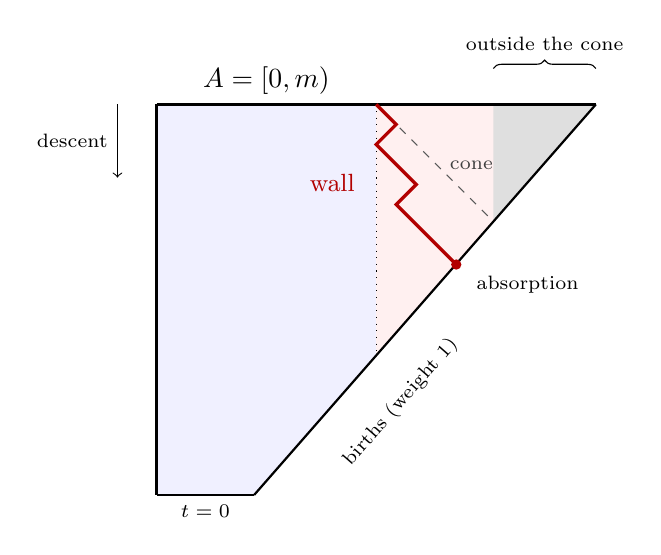
\begin{tikzpicture}[scale=0.62]
\fill[blue!6] (0,0) -- (2,0) -- (4.5,2.857) -- (4.5,8) -- (0,8) -- cycle;
\fill[red!6] (4.5,8) -- (9,8) -- (4.5,2.857) -- cycle;
\fill[gray!25] (6.9,5.6) -- (9,8) -- (6.9,8) -- cycle;
\draw[thick] (0,0) -- (0,8);
\draw[thick] (2,0) -- (9,8);
\draw[thick] (0,8) -- (9,8);
\draw[thick] (0,0) -- (2,0);
\draw[dotted] (4.5,8) -- (4.5,2.857);
\node[above] at (2.25,8) {$A=[0,m)$};
\node[above] at (5.7,8) {$\Abar$};
\draw[dashed,gray!70!black] (4.5,8) -- (6.9,5.6);
\node[gray!50!black,font=\scriptsize] at (6.45,6.75) {cone};
\draw[decorate,decoration={brace,amplitude=3pt,raise=13pt}] (6.9,8) -- (9,8) node[midway,above=16pt,font=\scriptsize] {outside the cone};
\draw[very thick,red!70!black] (4.5,8) -- (4.91,7.59) -- (4.5,7.18) -- (4.91,6.77) -- (5.32,6.36) -- (4.91,5.95) -- (5.32,5.54) -- (5.73,5.13) -- (6.14,4.72);
\fill[red!70!black] (6.14,4.72) circle (3pt);
\node[red!70!black,font=\small] at (3.6,6.4) {wall};
\node[font=\scriptsize,rotate=48.8] at (5.0,1.9) {births (weight $1$)};
\node[font=\scriptsize] at (7.6,4.3) {absorption};
\draw[->] (-0.8,8) -- (-0.8,6.5); \node[left,font=\scriptsize] at (-0.8,7.25) {descent};
\node[below,font=\scriptsize] at (1,0) {$t=0$};
\end{tikzpicture}
\caption{Edge growth in one dimension. Theorem~A bounds $G$ from below by the number of qudits of $\Abar$ born after the cone has passed (grey area): their world lines do not meet the causal past of $A$. For gates drawn from a 2-design, the average purity is a sum over the walks of a single wall (Proposition~\ref{prop:single}). The wall starts at the cut, makes $\pm1$ steps of weight $K$, and stops on the line of births, on the left edge, or at $t=0$.}
\label{fig:wall}
\end{figure}

\subsection{Exponential martingale}

\begin{lemma}[weight identity]\label{lem:weights}
For $j$ steps to the right and $l$ steps to the left, $K^{j+l}=q^{-(j-l)}\,a^j b^l$ (Coq: \texttt{weight\_identity}).
\end{lemma}

Let $\mathbb{P}_a$ be the law of the walk that moves right with probability $a$ and left with probability $b$ under each gate. Its velocity is $v_B$: it is the walk of the front of a spreading operator \cite{NVH2018,vK2018}. Let $X$ be the net displacement, counted only over the steps made under a gate, up to absorption or up to $t=0$.

\begin{corollary}[probabilistic representation]\label{cor:proba}
Exactly, $Z_A=\E_a\bigl[q^{-X}\bigr]=\E_b\bigl[q^{\,X}\bigr]$.
\end{corollary}
\begin{proof}
Each walk $\omega$ has weight $K^{j+l}=\mathbb{P}_a(\omega)\,q^{-X(\omega)}$ (Lemma~\ref{lem:weights}). The second form follows by exchanging $a$ and $b$.
\end{proof}

\begin{lemma}[bundle]\label{lem:bundle}
(a) $\binom{j+l}{j}K^{j+l}\le q^{-|j-l|}$ (Coq: \texttt{path\_bundle}, via the binomial identity $(a+b)^{j+l}=1$).
(b) The total weight of all paths of $t$ steps is $(2K)^t=e^{-tE(0)}\le1$ (Coq proof of $2K\le1$: \texttt{twoK\_le\_1}).
(c) $\binom{t}{j}K^t\le e^{-tE((2j-t)/t)}$, from the elementary bound $\binom tj\le e^{t\,h(j/t)}$ and $(1+v)/2=j/t$.
\end{lemma}

\subsection{Theorem D: recent births count the deficit}

Let $B(t)$ be the number of births with date $L\ge T-t$, i.e.\ during the last $t$ layers, endpoints included.

\begin{theoremL}\label{thm:D}
Assume a brickwork circuit, independent gates drawn from a 2-design, births at the right edge at arbitrary dates, and $A=\{0,\dots,m-1\}$ with $N-m\ge m$. Let $t^\ast=\lceil m\log q/E(0)\rceil=\lceil m/v_E^{(2)}\rceil$. If $T\ge t^\ast$, then
\begin{equation}\label{eq:thD}
Z_A\le\Bigl(2+\frac{1}{2K}\Bigr)\,q^{-(m-B(t^\ast))},\qquad
\E[G(A)]\le\log q\cdot B(t^\ast)+\log\Bigl(2+\frac{q^2+1}{2q}\Bigr).
\end{equation}
For $q=2$ the constant is $\log_2 3.25=1.70$ bits.
\end{theoremL}

The proof (Appendix~\ref{app:D}) classifies the walks by their stopping time: walks absorbed on the right before $t^\ast$ have travelled at least $m-B(t^\ast)$ sites and are suppressed by Corollary~\ref{cor:proba}; walks absorbed on the left are suppressed by $q^{-m}$; walks still alive after $t^\ast$ layers are suppressed by $(2K)^{t^\ast-1}$ (Lemma~\ref{lem:bundle}(b)).

\begin{proposition}[lower bound, every circuit]\label{prop:lower}
With births at the right edge and for every $s$ such that $s+B(s)\le m$, $G(A)\ge\log q\cdot B(s)$ for \emph{every} circuit.
\end{proposition}
\begin{proof}
The right edge of the causal past of $A$ moves by at most one site per layer; at date $L$ it lies at most at $m-1+(T-L)$. The births of the last $s$ layers occupy positions $x\ge N-B(s)\ge 2m-B(s)$, since $N\ge 2m$. They are outside the cone as soon as $2m-B(s)>m-1+s$, and they belong to $\Abar$. Conclude with Theorem~A.
\end{proof}

Thus $\log q\cdot B(\approx m)\le G$ and $\E[G]\le\log q\cdot B(m/v_E^{(2)})+O(1)$. For a 2-design dynamics, the mean deficit is bracketed by the births of two recent windows. The first lasts the light-crossing time ($m$ layers), the second the entanglement-crossing time ($m/v_E^{(2)}$, i.e.\ $3.11\,m$ for $q=2$). Older births have been ``digested''; more recent ones cannot be. This is a quantitative analogue, for this model, of Frautschi's horizon argument.

\begin{corollary}[summation for $\alpha<1$]\label{cor:alpha}
Consider births at the right edge with $n(L)-N_0=\lfloor L^\alpha\rfloor$, $0<\alpha<1$, and a final time $T$ such that $N=2m$. There are constants $C,c>0$, depending on $q$ and $\alpha$, such that for $m$ large enough
\begin{equation}
c\,m^{2-1/\alpha}-\log q\le\E[G(A)]\le C\,m^{2-1/\alpha}+C\quad(\tfrac12<\alpha<1),\qquad
\E[G(A)]\le C\quad(\alpha\le\tfrac12).
\end{equation}
In particular $\E[G]/N\to0$, and the exponent $2-1/\alpha$ is exact.
\end{corollary}
\begin{proof}
One has $T\simeq(2m-N_0)^{1/\alpha}\gg m$, so $t^\ast\le T/2$ for large $m$. By concavity, $B(t)\le T^\alpha-(T-t)^\alpha+1\le\alpha t(T/2)^{\alpha-1}+1$ for $t\le T/2$; with $t=t^\ast=O(m)$, Theorem~D gives the upper bound. For the lower bound, $B(s)\ge\alpha sT^{\alpha-1}-1$; take $s=\lfloor m/2\rfloor$, which satisfies $s+B(s)\le m$ for large $m$, and apply Proposition~\ref{prop:lower}.
\end{proof}

For $\alpha\le\frac12$, $m\log q-\Srec\to\log 2$ (Figure~\ref{fig:alpha}). This is the annealed Page correction \cite{Page1993}: $Z_A\simeq 2q^{-m}$, with one term from absorption on the right and one from absorption on the left, each of order $q^{-m}$.

\subsection{Theorem E: exact annealed density at $\alpha=1$}

\begin{theoremL}\label{thm:E}
Consider one birth every $k$ layers, as in Section~\ref{sec:A1}, with $N=2m$. Let $\theta_k\in(0,\log q)$ be the unique positive root of
\begin{equation}\label{eq:theta}
2K\cosh\theta=e^{-\theta/k}.
\end{equation}
Then, for $m$ large enough, $\tfrac12 e^{-2\theta_k}\,e^{-\theta_k m}\le Z_A\le (e^{2\theta_k}+2)\,e^{-\theta_k m}$, that is $\Srec(A)=\theta_k\,m+O(1)$. Moreover:
(a) $\theta_k=\min_{0\le v\le1}E(v)/(v+1/k)$;
(b) $\theta_1=\frac12\log\frac{q^2-q+1}{q}$, i.e.\ $0.2925$ bit per qudit for $q=2$ (Coq: \texttt{theta1\_root});
(c) $\theta_k<\log q\cdot\frac{kv_B}{1+kv_B}<\log q\cdot\frac{k}{k+1}$, and $\theta_k\to\log q$ as $k\to\infty$.
\end{theoremL}

The proof (Appendix~\ref{app:E}) uses the exponential martingale $h(D)=e^{-\theta_kD}$, where $D$ is the number of living legs to the right of the wall: \eqref{eq:theta} is exactly the condition for $h$ to be invariant under one period (one birth and $k$ layers) of the descent. Part (a) says that $\theta_k$ is the minimal cost of a wall that ends on the line of births, the exact counterpart, with an inclined absorbing boundary, of the membrane picture of \cite{ZhouNahum2019,ZhouNahum2020}.

\begin{proposition}[closed form for $k=1$]\label{prop:k1}
For $k=1$, $Z_A=\bigl(\frac{K}{1-K}\bigr)^{j^\ast}(1+O(e^{-cm}))$, where $j^\ast=m/2$ if $m$ is even and $j^\ast=(m\pm1)/2$ if $m$ is odd, depending on the phase of the first layer.
\end{proposition}
\begin{proof}
At $k=1$, each step back consists of one layer and one removal: $D$ decreases by $2$ (right step) or stays the same (left step). Absorption on the right happens at the $j^\ast$-th right step, and the negative binomial series gives $\sum_l\binom{j^\ast-1+l}{l}K^{j^\ast+l}=(K/(1-K))^{j^\ast}$. The excluded terms and the left and surviving contributions are exponentially smaller.
\end{proof}

\begin{corollary}[bracket at $\alpha=1$]\label{cor:bracket}
For gates drawn from a 2-design,
\begin{equation}\label{eq:bracket}
\frac{m-\mathcal{E}_k(m)}{2m}\le\frac{\E[G]}{N\log q}\le\frac12\Bigl(1-\frac{\theta_k}{\log q}\Bigr)+O\Bigl(\frac1m\Bigr),\qquad N=2m .
\end{equation}
The left bound tends to $\frac1{2(1+k)}$, holds for every circuit, and is attained (Proposition~\ref{prop:A1}). The right bound follows from Theorem~E and \eqref{eq:jensen}. As $q\to\infty$, $\theta_k/\log q\to k/(k+1)$ and the bracket closes on the minimal cut.
\end{corollary}

\begin{table}[h]
\centering\footnotesize\setlength{\tabcolsep}{4.5pt}
\begin{tabular}{c|cccc|cccc}
\toprule
 & \multicolumn{4}{c|}{$\theta_k/\log q$} & \multicolumn{4}{c}{bracket of $\E[G]/(N\log q)$} \\
$q$ & $k=1$ & $2$ & $4$ & $8$ & $k=1$ & $2$ & $4$ & $8$\\
\midrule
2 & 0.2925 & 0.4843 & 0.6760 & 0.8168 & [0.250, 0.354] & [0.167, 0.258] & [0.100, 0.162] & [0.056, 0.092]\\
3 & 0.3856 & 0.5814 & 0.7480 & 0.8603 & [0.250, 0.307] & [0.167, 0.209] & [0.100, 0.126] & [0.056, 0.070]\\
10 & 0.4795 & 0.6558 & 0.7946 & 0.8863 & [0.250, 0.260] & [0.167, 0.172] & [0.100, 0.103] & [0.056, 0.057]\\
\bottomrule
\end{tabular}
\caption{Values of $\theta_k$ (Theorem~E) and the bracket \eqref{eq:bracket} as $m\to\infty$.}
\label{tab:theta}
\end{table}

\begin{remark}[finite-size corrections]\label{rem:finitesize}
Theorem~E bounds the correction $c(m)=-\ln Z_A-\theta_km$ by $-\ln(e^{2\theta_k}+2)\le c(m)\le2\theta_k+\ln2$. The exact recursion ($q=2$; $k=1,2,4,8$; $N_0\in\{2,4,10\}$; $8\le m\le4097$) says more.
\begin{itemize}[leftmargin=*,itemsep=1pt]
\item $c(m)$ converges exponentially fast: $|c(m)-c(\infty)|<10^{-6}$ at the latest from $m=48$ ($k=1$), $49$ ($k=2$), $65$ ($k=4$) and $129$ ($k=8$), for the three values of $N_0$ and both parities of $m$.
\item The limit depends on the parity of $m$ but not on $N_0$. In nats: $c(\infty)=0$ and $-\theta_1$ for $k=1$ ($m$ even, odd), in agreement with Proposition~\ref{prop:k1}; $0.138$ and $-0.029$ for $k=2$; $0.199$ and $0.082$ for $k=4$; $0.249$ and $0.178$ for $k=8$.
\item The subleading constant is thus \emph{not universal}: it depends on microscopic details (the phase of the pattern when the wall arrives), while remaining bounded and small. The relative error on the density, $|{-\ln Z_A}/(\theta_km)-1|$, falls below $1\,\%$ from $m=33$ for $k\ge2$ and from $m=128$ for $k=1$ (because of odd $m$).
\end{itemize}
\end{remark}

\begin{remark}[membrane estimate]\label{rem:membrane}
A non-rigorous two-path estimate from the theory of entanglement membranes \cite{JHN2018,ZhouNahum2020} gives $dG/dN\gtrsim\frac12\max(1-kv_E,\,1/(1+kv_B))$: it compares the horizontal membrane (cost $v_E$ per layer) with the membrane that follows the front of an operator down to the line of births. The algebra of this estimate is checked in Coq (\texttt{ConeLemmas.v}); its premises, entropy bounded by the cost of each cut, are not. For a 2-design and the annealed tension, Theorem~E replaces the two extreme paths by the optimal one, $\min_vE(v)/(v+1/k)$. The same formula with an unknown quenched tension, convex and tangent at $v_B$, would give the unproven bracket $kv_E/(1+kv_E)\le\E[S]/m\le\min(kv_E,\,v_Bk/(1+v_Bk))$, in bits.
\end{remark}

\begin{remark}[structured dynamics]\label{rem:dualunit}
Theorems~D and~E assume a 2-design. Exploratory runs, \emph{not pre-registered}, on dual-unitary Clifford circuits ($\mathrm{SWAP}\cdot\mathrm{CZ}$ dressed with single-qubit gates) show that the position inside the bracket depends on the dressing. With random single-qubit dressing, $G=G_{\rm LB}$ exactly in $48$ points out of $48$ (edge growth, $k=1,\dots,4$, $N\le800$), so the lower bound is attained by a natural dynamics. The deterministic dressings $\mathrm{SWAP}\cdot\mathrm{CZ}$ and $\mathrm{SWAP}\cdot\mathrm{CZ}\cdot(H\otimes I)$ leave instead an extensive extra deficit; in the first case, qudits born in $|0\rangle$ are invariant under $\mathrm{CZ}$. Dual unitarity and maximal entangling power are therefore not enough: what matters is how the dynamics acts on the birth states.
\end{remark}
